\documentclass[journal]{IEEEtran}
\usepackage{amsthm}
\usepackage{url}
\usepackage{graphicx}
\usepackage{listings}
\usepackage{color}

\definecolor{dkgreen}{rgb}{0,0.6,0}
\definecolor{gray}{rgb}{0.5,0.5,0.5}
\definecolor{mauve}{rgb}{0.58,0,0.82}

\lstset{frame=tb,
  language=SQL,
  aboveskip=3mm,
  belowskip=3mm,
  showstringspaces=false,
  columns=flexible,
  basicstyle={\small\ttfamily},
  numbers=none,
  numberstyle=\tiny\color{gray},
  keywordstyle=\color{blue},
  commentstyle=\color{dkgreen},
  stringstyle=\color{mauve},
  breaklines=true,
  breakatwhitespace=true,
  tabsize=3
}
\begin{document}

\title{SQLi Prevention System}
\author{

Shreyans Soni\\
2016CSB1146@iitrpr.ac.in

}

\maketitle
\begin{abstract}
 My Project is about making such a framework or a PHP filter which prevent SQL injection from happening. In simple ways I want to create such mechanism which blocks the malicious SQL quries from the user side and take appropriate actions. 

\end{abstract}

\section{Introduction}
  What is a SQL injection in the first place?.
  Let's understand first the terms than we will dive into the depths of the project.
\subsection{SQL}
 SQL stands for "Structured Query Language".
 SQL is a standard language for storing, manipulating and retrieving data in databases.\\
 example of a SQL query is as follows.
 \begin{lstlisting}
 SELECT col1, col2, col3...
FROM table_name1, table_name2 
WHERE table_name1.col2 = table_name2.col1;
 \end{lstlisting}
 which extracts col1,col2,col3 from table 1 and 2 on certain conditions.
\subsection{SQLi}
 SQL Injection (SQLi) refers to an injection attack wherein an attacker can execute malicious SQL statements (also commonly referred to as a malicious payload) that control a web application’s database server (also commonly referred to as a Relational Database Management System – RDBMS). Since an SQL Injection vulnerability could possibly affect any website or web application that makes use of an SQL-based database, the vulnerability is one of the oldest, most prevalent and most dangerous of web application vulnerabilities.\\
 a simple example of a SQLi query is as follows.
 \begin{lstlisting}
 SELECT id FROM users WHERE username=’username’ AND password=’password’ OR 1=1’
 \end{lstlisting}
 the working of such query grants user access to database see Figure~\ref{fig:block-diagram}
 
 \section{Why it is important}
 The main question is why it is so important and serious issue for a programmer/developers.
 The power which SQL contains has both sides of coins,an attacker can use this as follows:
 \begin{itemize}
     \item An attacker can use SQL Injection to bypass authentication or even impersonate specific users.
\item One of SQL’s primary functions is to select data based on a query and output the result of that query. An SQL Injection vulnerability could allow the complete disclosure of data residing on a database server.
\item Since web applications use SQL to alter data within a database, an attacker could use SQL Injection to alter data stored in a database. Altering data affects data integrity and could cause repudiation issues, for instance, issues such as voiding transactions, altering balances and other records.
\item SQL is used to delete records from a database. An attacker could use an SQL Injection vulnerability to delete data from a database. Even if an appropriate backup strategy is employed, deletion of data could affect an application’s availability until the database is restored.
\item Some database servers are configured (intentional or otherwise) to allow arbitrary execution of operating system commands on the database server. Given the right conditions, an attacker could use SQL Injection as the initial vector in an attack of an internal network that sits behind a firewall.
 \end{itemize}
 
\section{Technical Approach}
The approach for making such a mechanism is as follows:
\begin{itemize}
\item Collecting all the data From security forums for recognizing SQLi pattern
\item Selecting that data for a certain security level(as there are many types and levels of SQLi attacks). 
\item Designing a web based filter which filters all the client side queries.\cite{boyd2004sqlrand}
\end{itemize}

\begin{figure}
\centering
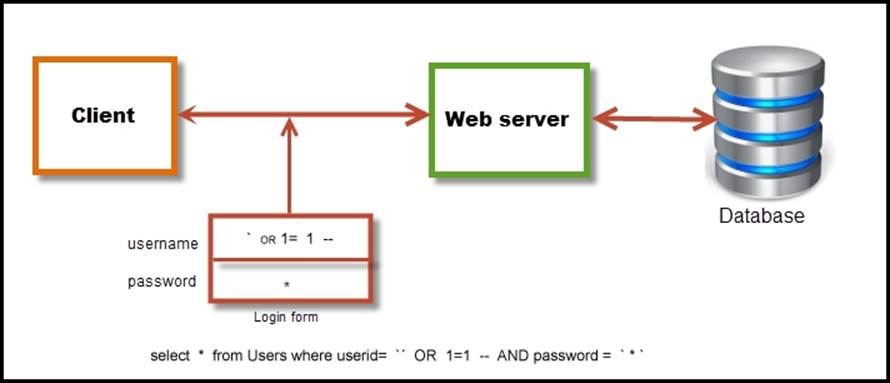
\includegraphics[width=1\linewidth]{sql.jpg}
\caption{Block diagram of malicious SQL query on a server.}
\label{fig:block-diagram}
\end{figure}
%Adding * spans the figure over two columns.


\section{Further Work}
Further plans for this project is that I want to extend this project not only for preventing the SQLi vulnerability but also for other top web based vulnerability such as XSS,CSFR,LFI etc..\\
Also this project can also befurther extended to the Android Systems as android also uses databases for maintaining the data which is handled by the SQL lite.
I am citing a document for SQL injection.
\cite{halfond2006classification}

\bibliographystyle{abbrv}
\bibliography{reference} 
\end{document}


